\documentclass[a4paper,oneside]{article}
\usepackage[utf8]{inputenc}	
\usepackage[T1]{fontenc}
\usepackage[ngerman]{babel}



%\usepackage{palatino}
%\renewcommand{\familydefault}{\sfdefault}

%\usepackage{amsmath}
\usepackage{amsfonts}
\usepackage{amssymb}
\usepackage{braket}
\usepackage[fleqn]{amsmath}

\usepackage{pgf,pgfarrows,pgfnodes}

\usepackage{mathptmx}
\usepackage{microtype}
\usepackage[nice]{nicefrac}

\usepackage{booktabs}

\usepackage{graphicx}

\usepackage{hyperref}

\usepackage{url}


%\setcounter{tocdepth}{2}
%\setkomafont{captionlabel}{\upshape\bfseries}
%\setkomafont{caption}{\itshape}

\usepackage{textcomp}

\usepackage{floatflt}

\title{Laserspektroskopie}
\author{
Benjamin Seeber\\
\vspace{25pt}
seeberbenjamin@googlemail.com\\
Thierry Fredrich\\
Thierry.Fredrich@googlemail.com
}

\date{31. August - 11. September 2009}

\begin{document}
\begin{titlepage}
  \maketitle
  \vfill
  \thispagestyle{empty}



\begin{abstract}
???
\end{abstract}
\end{titlepage}


\tableofcontents
\clearpage

\section{Einleitung}
Worum geht es, weiss man besser später
\subsection{Laser}
Der Laser ist heutzutage ein unverzichtbares Hilfsmittel der experimentellen Physik. Seine Einsatzmöglichkeiten sind quasi unbegrenzt. Neben dem wichtigsten Beipiel, welches der Namensgeber für diesen Versuch war, sind die bekanntesten Einsaztgebiete die optische Fallen und (ultra-) kalte Atomen. \\
Trotz den zahlreichen Realisierungen ist das physikaliche Prinzip eines jeden Lasers immer das Gleiche.
\subsubsection{Physikaliches Prinzip}
Ziel ist es eine starke Abweichung von der thermischen Besetzungsverteilung der Zustände in einem \textbf{aktiven Medium} zu erreichen. Man spricht von der Besetzungsinversion, d.h. Zustände mit höherer Energie sind entgegen der thermische Besetzung bevölkerter als Zustände niedriger Energie (siehe Abb. \ref{besetzungsinversion}).\\

\begin{figure}[!htb]
 \centering
 \includegraphics[bb=0 0 271 169]{./pics/besetzungsinversion.png}
 % besetzungsinversion.png: 363x225 pixel, 72dpi, 12.80x7.94 cm, bb=0 0 363 225
 \caption[Besetzungsinversion (aus \cite{dem3})]{Selektive Besetzunginversion ($N_i>N_k$ trotz $E_i>E_k$) als Abweichung von der thermischen Besetzungsverteilung.(aus \cite{dem3})}
 \label{besetzungsinversion}
\end{figure}
Um dies zu erreichen muss man natürlich, da es nicht der Wille der Natur ist, Energie in das System stecken. Dies geschieht mit einer \textbf{Engergiepumpe}. Zu guter letzt brauchen wir noch einen \textbf{optischen Resonator}, der die vom aktiven Medium emitierte Fluoreszenz in wenigen Moden des Strahlungsfeldes speichert, so dass in diesen Moden die Photonenzahl groß wird und damit die induzierte Emission viel wahrscheinlicher als die spontane Emission wird. Der optische Resonator hat außerdem dei Aufgabe, die durch induzierte Emission verstärkte Strahlung in das aktive Medium zurückzuführen, so dass aus dem Lichtverstärker ein Lichtoszillator wird.
Man merke sich also: ein Laser braucht drei Dinge:\\


\begin{enumerate}
\item \textbf{aktives Medium}\\
\item \textbf{Energiepumpe}\\
\item \textbf{opitscher Resonator} 
\end{enumerate}

\subsubsection{Optischer Resonator}

Um eine Konzentration der induzierten Emission auf wenige Moden zu erreichen, muß die Speicherfähigkeit des Resonators für diese Mode groß sein, d.h. seine Verluste müssen klein sein, während für alle anderen Moden die Verluste so groß sein sollten, dass für sie bei gegebener Pumpleistung die Schwelle zur Laseroszillation nicht erreicht wird.\\
Offene optische Resonatoren, die aus geeignet dimensionierten Anordungen von Spiegeln bestehen, können die obigen Bedingungen in idealer Weise erfüllen. Für den hier realisierten Laser wären die Beugungsverlust bei Verwendung ebener Spiegel viel zu hoch. Deshalb verwendet man sphärische Spiegel. Kippt man einen ebenen Spiegel um den Winkel $\epsilon$, so wird der reflektierte Strahl um $2\epsilon$ verkippt,so daß schon bei kleinen Werten für $\epsilon$ der Strahl nach wenigen Resonatorumläufen das verstärkende Medium nicht mehr durchlaufen kann.\\
Bei einem sphärischen Spiegel führt eine Verkippung um den gleichen Winkel $\epsilon$ insgesamt zu einem wesentlich kleineren Strahlverlust. Man sprich von einen \textbf{konfokalen Resonator} (wie er bei uns zum Einsatz kommt), wenn die Krümmungsradien ($r_1, r_2$) der beiden Spiegeln gerade deren Abstand ($d$) entspricht.

\begin{equation*}
r_1=r_2=d
\end{equation*}

Deshalb können wir die folgende Diskussion auf paraxiale Strahlen beschränken. Es können sich stehende Wellen im Resonator ausbilden, wenn 
\begin{equation}
 d=q\cdot \frac{\lambda}{2} \text{\;\;\;\;ODER\;\;\;\;} \nu_r=q\cdot \frac{c}{2d} \text{\;\;\;mit }q\in \mathbb{N} 
 \label{bediengung_fuer_stehende_welle}
\end{equation}

gilt. Der \textbf{freie Spektralbereich} eines Resonator ist definiert als die Differez zweier Resonazfrequenz, was nach (\ref{bediengung_fuer_stehende_welle}) gerade:
\begin{equation}
 \delta \nu_r=\frac{c}{2d}
\end{equation}
ist. Auf Grund von Reflexionsverlusten an den Spiegeln haben die Transmissionslinien eine endliche Halbwertsbreite $\delta f$. Die Finesse $F$ eines Resonators ist ein Maß für die Anzahl der Umläufe eines Photons im Resonator. Sie hängt also direkt von der Reflektivität der Spiegel ab und berechnet sich über den Quotienten von freiem Spektralbereich und Halbwertsbreite:
\begin{equation}
 F=\frac{\delta \nu_r}{\delta f}
\end{equation}

\subsubsection{Frequenzmodulation}
\label{theorie_fm}
Das Lichtfeld der Laserdiode mit der Kreisfrequenz $\omega_0$ lässt sich durch


\begin{align}
E(t)  &=E_0\cos(\omega_0t)\\ 
  &=\frac{E_0}{2}(e^{i\omega_0t}+e^{-i\omega_0t})
\end{align}

beschreiben. Dabei ist die Kreisfrequenz proportional zum Laserdiodenstrom. Moduliert man den Strom periodisch mit der Modulationsfrequenz $\omega_M$:

\begin{equation}
 I(t)=I_0+I_M\sin(\omega_Mt)
\end{equation}

so bewirkt dies eine Frequenz- bzw. Phasenmodulation des Lasers:

\begin{equation}
 E(t)=\frac{E_0}{2}e^{i(\omega_0t+\sin(\omega_Mt))}+c.c.
\end{equation}

Der Modulationsindex $M$ ist eine dimensionslose Größe und hier proportional zu $I_M$. Die momentane Phase (das Integral über die Kreisfrequenz) ist
\begin{equation*}
 \psi(t)=\omega_0t+M\sin(\omega_Wt)
\end{equation*}

Wir untersuchen den Term $e^{iM\sin(\omega_Mt)}$ etwas genauer. Es gilt:
\begin{align}
 e^{iM\sin(\omega_Mt)}&=e^{\frac{iMx}{2}}\cdot e^{\frac{-iMx}{2}}\\
&=\sum_{r=0}^{\infty} \left(\frac{M}{2}\right)^r\frac{x^r}{r!}\sum_{s=0}^{\infty} (-1)^s\left(\frac{M}{2}\right)^s\frac{x^{-s}}{s!}\\
&=\sum_{n=-\infty}^{\infty}J_n(M)x^n
\end{align}

Die Koeffizienten $J_n$ heißen $n$-te Besselfunktionen und haben folgende Gestalt:

\begin{figure}[!htb]
 \centering
 \includegraphics[bb=0 0 300 156]{./pics/Bessel.eps}
 % Bessel.eps: 0x0 pixel, 300dpi, 0.00x0.00 cm, bb=0 0 300 156
 \caption{Intensität der ersten 3 Besselfunktionen}
 \label{bessel}
\end{figure}


\begin{equation}
 J_n=\sum_{s=0}^\infty \frac{(-1)^s}{s!(n+s)!}\left(\frac{M}{2}\right)^{n+2s}
\end{equation}
In Abbildung \ref{bessel} ist zur Veranschaulichung ihr Betragsquadrat geplottet.
Für das $E$-Feld folgt also:
\begin{equation}
 E(t)=\frac{E_0}{2}e^{i\omega_0t}\sum_{n=-\infty}^\infty J_n(M) e^{in\omega_Mt)}+c.c.
\end{equation}

Das Lichtfeld setzt sich also aus Komponenten $\omega_0\pm n\omega_M$ zusammen. Siehe dazu Abb. \ref{schema_fm}.
\begin{figure}[!htb]
 \centering
 \includegraphics[bb=0 0 169 169]{./pics/fm_schema.png}
 % fm_schema.png: 225x225 pixel, 96dpi, 5.95x5.95 cm, bb=0 0 169 169
 \caption[FM- Spektrum]{Schema des FM- Spektrums bei konstantem $\omega_M$ und wachsendem $M$}
 \label{schema_fm}
\end{figure}
Ist $M\ll1$ (also eine kleine Amplitude der Modulation), so kann man die zweite $e$- Funktion entwickeln und es gilt:
\begin{align}
 E(t)&=E_0\cdot e^{i\omega_0 t}\cdot e^{iM\sin(\omega_M t)}+c.c.\nonumber\\
&\approx E_0\cdot e^{i\omega_0 t}\cdot(1+iM\sin(\omega_M t))+c.c\nonumber\\
&=E_0\cdot e^{i\omega_0 t}(1-\frac{M}{2}e^{-i\omega_Mt}+\frac{M}{2}e^{+i\omega_Mt})+c.c.\nonumber\\
&=E_0\cdot(e^{i\omega_0 t}-\frac{M}{2}e^{-i(\omega_0-\omega_M)t}+\frac{M}{2}e^{+i(\omega_0-\omega_M)t})+c.c.
\end{align}
Man erhält also ein Frequenzspektrum mit einem starken Träger bei der Frequenz $\omega_T$ und zwei schwachen Seitenbändern bei den Frequnzen $\omega_T\pm\omega_M$. Wir schicken nun das Laserlicht dieses Frequnzspektrums durch den Resonator oder die Zelle. Der Resonator transmitiert nur die Frequenzen seiner atomaren Res

\subsubsection{Halbleiterlaser}
\begin{figure}[!htb]
 \centering
 \includegraphics[bb=0 0 244 157]{./pics/schema_pn.png}
 \caption[Halbleiterlaser]{Vereinfachter schematischer Aufbau eines Halbleiterlasers (aus \cite{dem3})}
 \label{schema_pn}
 % schema_pn.png: 406x262 pixel, 72dpi, 14.32x9.24 cm, bb=0 0 406 262
\end{figure}

In dem hier durchgeführten Versuch werden wir einen Halbleiterlaser verwenden. Hier dient ein $p-n$-Diode, die in Durchlaßrichtung von einem Strom $I_D$ durchflossen wird, als aktives Medium (siehe Abb. \ref{schema_pn}). Im Übergangsgebiet zwischen dem n-Teil, in dem Elektronenüberschuß herrscht, und dem p- Teil, der einen Elektronenmangel und deshalb nicht besetzte Zustände (Löcher) hat, können die Elektronen aus einem energetisch höheren Zustand im Leitungsband in diese freien Zustände mit tieferer Energie fallen. Das bei der Elektronen- Loch- Rekombination emittierte Licht kann beim Durchgang durch die $p-n$-Grenzschicht verstärkt werden. Wegen der großen Elektronendichte ist die Verstärkung pro Weglänge sehr groß, und es genügen Längen unter $1 mm$, um die Laserschwelle zu überschreiten.\\
Der Spektralbereich der spontanen Emission ist abhängig von der Differenz der Energiebänder der beteiligten Niveaus und kann daher mittel aller Parameter, die den Abstand der Bänder beeinflussen (siehe Halbleiterphysik) durchgestimmt werden.
\begin{figure}
 \centering
 \includegraphics[bb=0 0 292 169]{./pics/energieschema_halbleiterlaser.png}
 % energieschema_halbleiterlaser.png: 417x242 pixel, 72dpi, 14.71x8.54 cm, bb=0 0 417 242
 \caption{Energieniveauschema (aus \cite{dem3})}
\end{figure}

\subsubsection{Littmann- Anordnung}
Bei der Wellenlängendurchstimmung durch den Diodenstrom kommt es aber zu Temperatur-, Druck-, Brechungsindex-, und ... Änderungen. Aufgrund diese sehr unangenehmen Rückkopplungseffekte ist es auf diese einfache Weise nicht möglich einen echten durchstimmbares Frequenzspektrum zu erhalten.\\
Was wäre nun ein echte Experimentator, wenn er sich von diesen Schwierigkeiten abhalten lassen würde? Statt dessen bedienen wir uns der ``Littmann''-Anordnung. Statt der Endflächen der Laserdiode benutzen wir äußere Resonatorspiegel, deren Abstand man kontrolliert verändern kann. Wegen der dadurch bediengten größeren Resonatorlänge $L$ wird der Modenabstand kleiner, und man braucht zusätzlich wellenlängen- selektierende Elemente im Resonator, um den Einmoden- Betrieb zu erreichen.\\
Als typischer Aufbau eines solchen Halbleiterlasers mit einem externen Resonator ist in Abb \ref{littmann} die Littman- Anordnung gezeigt, bei welcher der Ausgangsstrahl aus der Halbleiterdiode $LD$ durch eine Linse zu einem aufgeweiteten parallelen Strahlbündel geformt wird, das streifend auf ein Reflexionsgitter fällt. Ist der Einfallswinkel gleich dem Ausfallswinkel so erhält man für die Wellenlängenselktieon folgende Formel:
\begin{equation}
 2d\sin(\alpha)=\lambda
\end{equation}
\begin{figure}[!htb]
 \centering
 \includegraphics[bb=0 0 337 256]{./pics/littmann.png}
 % littmann.png: 481x365 pixel, 72dpi, 16.97x12.87 cm, bb=0 0 481 365
 \caption[Littman- Anordung(aus \cite{deml})]{Durchstimmbarer Ein- Moden- Halbleiterlaser mit externem Resonator in einer Littmann- Anordnung (aus \cite{deml})}
 \label{littmann}
\end{figure}

\subsection{Lienienverbreiterung von Atomen}

\subsubsection{Natürliche Lienienbreite}
Sie ist ein echter QM- Effekt. Wie wir heute wissen, ist die konjugierte Größe zur Energie die Zeit. Aus der Fundamentalen Unschärferelation folgt dann direkt:
\begin{equation}
 \Delta E\cdot \Delta t\geq \hbar \;\;\;\;\;\;\;\;\;\;\;\;\Longrightarrow \;\;\;\;\;\;\;\;\;\;\;\;\nicefrac{\Delta E}{\hbar}\geq \frac{1}{\Delta t}=\Delta \nu
\end{equation}
und wir haben  ein Maß für die Lieneinenbreite gefunden. Warum sie natürlich heißt dürfte auch klar sein, denn die obigen Folgerungen haben direkten Bezug zur Quanteneigenschaft von Licht.\\
Bei einem Übergang $E_i\rightarrow E_k$ zwischen zwei angeregten Niveaus tragen beide Lebensdauern $\tau_i$ und $\tau_k$ zur natürlichen Lienienbreite bei, da die entsprechenden Energieunschärfen beider Niveaus sich addieren. Man erhält dann

\begin{eqnarray}
        & \Delta E &=\Delta E_i+\Delta E_k \nonumber\\
       \Rightarrow &\Delta \nu_n&= \frac{1}{2\pi}(\nu_i+\nu_k)
\end{eqnarray}


\subsubsection{Doppler- Verbreiterung}

Mit rein klassischen Mitteln ist es uns möglich die Doppler- Verbreiterung zu erklären. Bewegt sich ein angeregtes Atom mit o.B.d.A $\vec v=(0,0,v_z)$, so wird die Emitierte Frequenz $\omega_0$ des vom Atom in Richtung des Wellenvektor $\vec k=(0,0,k_z)$ emitierten Lichtes für einen ruhenden Beobachter infolge des Dopplereffektes verschoben zu:

\begin{equation}
 \omega_e=\omega_0+\vec k\cdot\vec v
\end{equation}

Auch die Absoptionsfrequenz $\omega_a$ eines Atoms, das sich mitder Geschwindigkeit $\vec v$ bewegt, ändert sich entsprechend. In unserem Beispiel ergibt sich eine Absorptionsfrequenz von :
\begin{equation}
 \omega_a=\omega_0+\vec k \vec v=\omega_0\left(1+\frac{v_z}{c}\right)
 \label{doppler_beziehung}
\end{equation}

Nutzt man jetzt die Hochtemperaturnäherung in welcher die Geschwindigkeitskomponenten maxwellsch verteilt sind, so kann man zeigen, dass Doppler-Halbwertsbreite gegeben ist durch die Formel
\begin{equation}
 \Delta \omega_{Doppler}=\left(\nicefrac{\omega_0}{c}\right)\sqrt{\nicefrac{8k_B T\cdot \ln(2)}{m}}
 \label{Doppler}
\end{equation}
Anzumerken gibt es hier, dass die Dopplerbreite $\Delta\omega_D$ linear mit der Frequenz $\omega_0$ ansteigt, mit steigender Temperatur $T$ proportional zu $\sqrt{T}$ zunimmt und mit zunehmender Masse $m$ wie $\frac{1}{\sqrt{m}}$ abnimmt.\\
Setzt man Zahlenwerten ein, so wird deutlich, dass die Dopplerverbreiterung im sichtbaren Gebiet die natürliche Linienbreite um etwa zwei Größenordnungen übertrifft.


\begin{figure}
 \centering
 \includegraphics[bb=0 0 220 145]{./pics/lorentz_vs_gauss.png}
 % lorentz_vs_gauss.png: 441x289 pixel, 72dpi, 15.56x10.19 cm, bb=0 0 441 289
 \caption[Gaus-und Lorentzkurve (aus \cite{dem3})]{Vergleich von Lorentzprofil und Gaußprofil mit gleicher Halbwertsbreit (aus \cite{dem3})}
 \label{lorentz_gauss}
\end{figure}

In Abb. \ref{lorentz_gauss} ist ein Vergleich der beiden Kurvenprofile dargestellt, der zeigt, dass die Lorentzkurve der natürlichen Linienbreite nach aussen hin wesentlich langsamer abfällt als der ``Schwanz'' der Gauss-Kurve.


\subsubsection{Druckverbreiterung}
Nähert sich Atom A einem anderen Atom B so werden sie früher oder später miteinander in Wechselwirkung treten. Diese Wechselwikung widerum wird dafür sorgen, dass ich die Energieniveaus der Konstituenten verschieben.\\
Eine Allgemein Aussage über die Effekte ist hier nicht möglich, da die Verbreiterung durch diese Stoßprozesse sehr individuell ist. Abhängen wird das Ganze aber von dem Abstand der Teilchen und von der Geschaffenheit ihrer Energieniveaus selber.\\
Unterschieben wird noch, ob die Moleküle von der selben Sorten sind (Eigendruckverbreiterung) oder ob es sich um unterschiedliche Atome (Fremddruckverbreiterung) handelt.

\subsection{Absoption von Licht}
bitte noch was schreiben!!!!!!!


\subsection{Polarisation von Licht}
\subsubsection{Jones- Vektoren}
Aus den Maxwell- Gleichung erhalten wir als Lösung ebene Wellen der Form
\begin{equation}
 \bf{E}=\bf{A_0}\;e^{i(\omega t-\bf{k}\cdot\bf{r})}
\end{equation}

Für eine in $z$-Richtung laufende Welle lässt sich der komplexe Amplitudenvektor $\textbf{A}_0$ schreiben als

%\begin{displaymath}\end{displaymath} is equivaltent to $$ $$ (good to know)


$$ \bf{A_0} = \left\{ \begin{array}{l}
A_{0x}\;e^{i\phi_x} \\
A_{0y}\;e^{i\phi_y}
\end{array} \right\} $$

Für unpolarisiertes Licht sind die Phasen $\phi_x$ und $\phi_y$ nicht korreliert und schwanken statistisch. Für linear plarisiertes Licht mit dem $\bf{E}$- Vektor in $x$- Richtung ist $A_{0y}=0$. Für linear plarisiertes Licht mit dem $\bf{E}$- Vektor in beliebige Richtung innerhalb der $xy$- Ebene gilt $\phi_x=\phi_y$, und das Verhältnis $\nicefrac{A_{0x}}{A_{0y}}$ gibt die Richtung von $\bf{E}$ an. Für zirkular polarisiertes Licht ist $A_{0x}=A_{0y}$ und $\phi_x=\phi_y\pm\frac{\pi}{2}$.\\
Für linear polarisiertes Licht, dessen $\bf{E}$-Vektor 45\textdegree gegen die $x$- Achse geneigt ist, gilt $\phi_x=\phi_y=\phi$ und
$$
\bf{A_{0}}=\sqrt{A_{0x}^2+A_{0y}^2}\frac{1}{\sqrt{2}}
\left\{ \begin{array}{l}
1 \\
1
\end{array} \right\}
=\left\|\bf{A_0}\right\|\frac{1}{\sqrt{2}}
\left\{ \begin{array}{l}
1 \\
1
\end{array} \right\}
$$
und für rechts zirkular polarisiertes $\sigma^-$-Licht haben wir wegen $e^{i\nicefrac{\pi}{2}}=-i$
\begin{equation}
 \bf{A_0}=\left\|\bf{A_0}\right\|\frac{1}{\sqrt{2}}
\left\{ \begin{array}{l}
1 \\
-i
\end{array} \right\}
\end{equation}
Man nennt diese Darstellung der Amplitude den \textbf{Jones- Vektor} und schreibt:
\begin{equation}
 E=
\left\{ \begin{array}{l}
E_x \\
E_y
\end{array} \right\}
=
\left\|\bf{E}\right\|
\left( \begin{array}{l}
a \\
b
\end{array} \right),
\end{equation}
wobei $a$, $b$ reelle oder komplexe Zahlen sind. Mithilfe der Jones- Vektoren lassen sich die Polarisationszustände des Lichtes übersichtlich schreiben (siehe Abb \ref{jonesvektoren}).
\begin{figure}
 \centering
 \includegraphics[bb=0 0 140 166]{./pics/jonesvektoren.png}
 % jonesvektoren.png: 279x332 pixel, 72dpi, 9.84x11.71 cm, bb=0 0 279 332
 \caption[Jones- Vektoren (aus \cite{deml})]{Jones Vektoren für in $z$-Richtung laufende Wellen (aus \cite{deml})}
 \label{jonesvektoren}
\end{figure}



\subsubsection{Jones- Operatoren}
Diese Jones- Darstellung erweist sich als vorteilhaft, wenn man den Druchgang von Licht durch optische Elemente betrachtet, die den Polarisationszustand verändern wie z.B. Strahlteiler, Polarisatoren oder doppelbrechende Kristalle. Beschreibt man diese Elemente durch zweireihige Matrizen, so erhält man den Polarisationszustand der transmittierten Welle durch Multiplikation des Jones- Vektors der einfallenden Welle mit der Jones- Matrix des Elementes:
$$
\left(
\begin{array}{l}
E_{xt}\\
E_{yt}
\end{array}
\right)
=
\left(
\begin{array}{ll}
a&b\\
c&d
\end{array}
\right)
\left(
\begin{array}{l}
E_{x0}\\
E_{y0}
\end{array}
\right)
$$
In Abb. \ref{jonesoperatoren} sind die Jones- Matrizen für einige optische Elemente angegeben.

\begin{figure}[h]
 \centering
 \includegraphics[bb=0 0 177 165]{./pics/jonesoperatoren.png}
 % jonesoperatoren.png: 354x331 pixel, 72dpi, 12.49x11.68 cm, bb=0 0 354 331
 \caption{Jones Matrizen für Polarisatoren (aus \cite{deml})}
 \label{jonesoperatoren}
\end{figure}

\subsection{Energieaufspaltung}
oder Verweis auf Literatur???

\subsection{Rubidium}
Rubidium (Rb) ist ein Alkalimetall, d.h. es besitzt ein einzelnes Elektron in seiner Außenschale und hat somit ein wasserstofähnliches Termschema. Es existieren zwei in der Natur vorkommende Isotope $^{85}$Rb mit $72\%$ und $^{87}$Rb mit $28\%$.\\
$^{85}$Rb ist ein stabiles Isotop und $^{87}$Rb zerfällt mit einer Halbwertszeit von $\sim 4\cdot 10^{10}$ Jahren über $\beta^-$ zu $^{87}$Sr (Strontium). Wegen der äußerst langen Halbwertszeit müssen allerdings keine besonderen Schutzmaßnahmen ergriffen werden. In unserem Versuch werden wir die $D_2$- Linie untersuchen.
\begin{figure}
 \centering
 \includegraphics[bb=0 0 405 319]{./pics/rubidium.gif}
 % rubidium.gif: 450x354 pixel, 72dpi, 15.88x12.49 cm, bb=0 0 450 354
 \caption[Rudidium von \cite{rub2}]{Energieschema von Rudidium von \cite{rub2}}
 \label{Energieschema_von_rubidium}
\end{figure}

\paragraph*{Spektroskopische Notation}
\begin{equation}
 n^{2S+1}L_J
\end{equation}
mit den üblichen Bezeichungen:

\begin{description}
 \item[n]=Hauptquantenzahl
 \item[S]=Elektronenspin
 \item[L]=Bahndrehimpuls
 \item[J]=Gesamtdrehimpuls
\end{description}
$D_2$-Linie bedeutet der Übergang von $5^2S_{\nicefrac{1}{2}}\;\longrightarrow\;5^2P_{\nicefrac{3}{2}}$.
Um diesen zu treiben, muss man Laserlicht mit einer Wellenlänge von $780,2nm$ einstrahlen (siehe Abb. \ref{Energieschema_von_rubidium}). Es tritt auch eine Isotopenverschiebung auf, d.h. die beiden Grundzustände $^{85}Rb 5^2S_{\nicefrac{1}{2}}$ und $^{87}Rb 5^2S_{\nicefrac{1}{2}}$ liegen nicht auf den gleichen Energieniveau.


%\begin{figure}
 %\centering
 %\includegraphics[width=\textwidth]{./pics/Rb_energy.eps}
 % Rb_energy.eps: 0x0 pixel, 300dpi, 0.00x0.00 cm, bb=14 14 626 806
%\end{figure}




\section{Experiment am Laser}
Um uns zunächst mit dem Laser vertraut zu machen, werden wird die Laserschwelle bestimmen und anschließend die Leistungs-Dioden-Kennlinie aufnehmen.
\subsection{Versuchsaufbau}
Der Aufbau ist sehr simpel und in Abb. \ref{Photodiodeneichung} dargestellt.

\begin{figure}
 \centering
 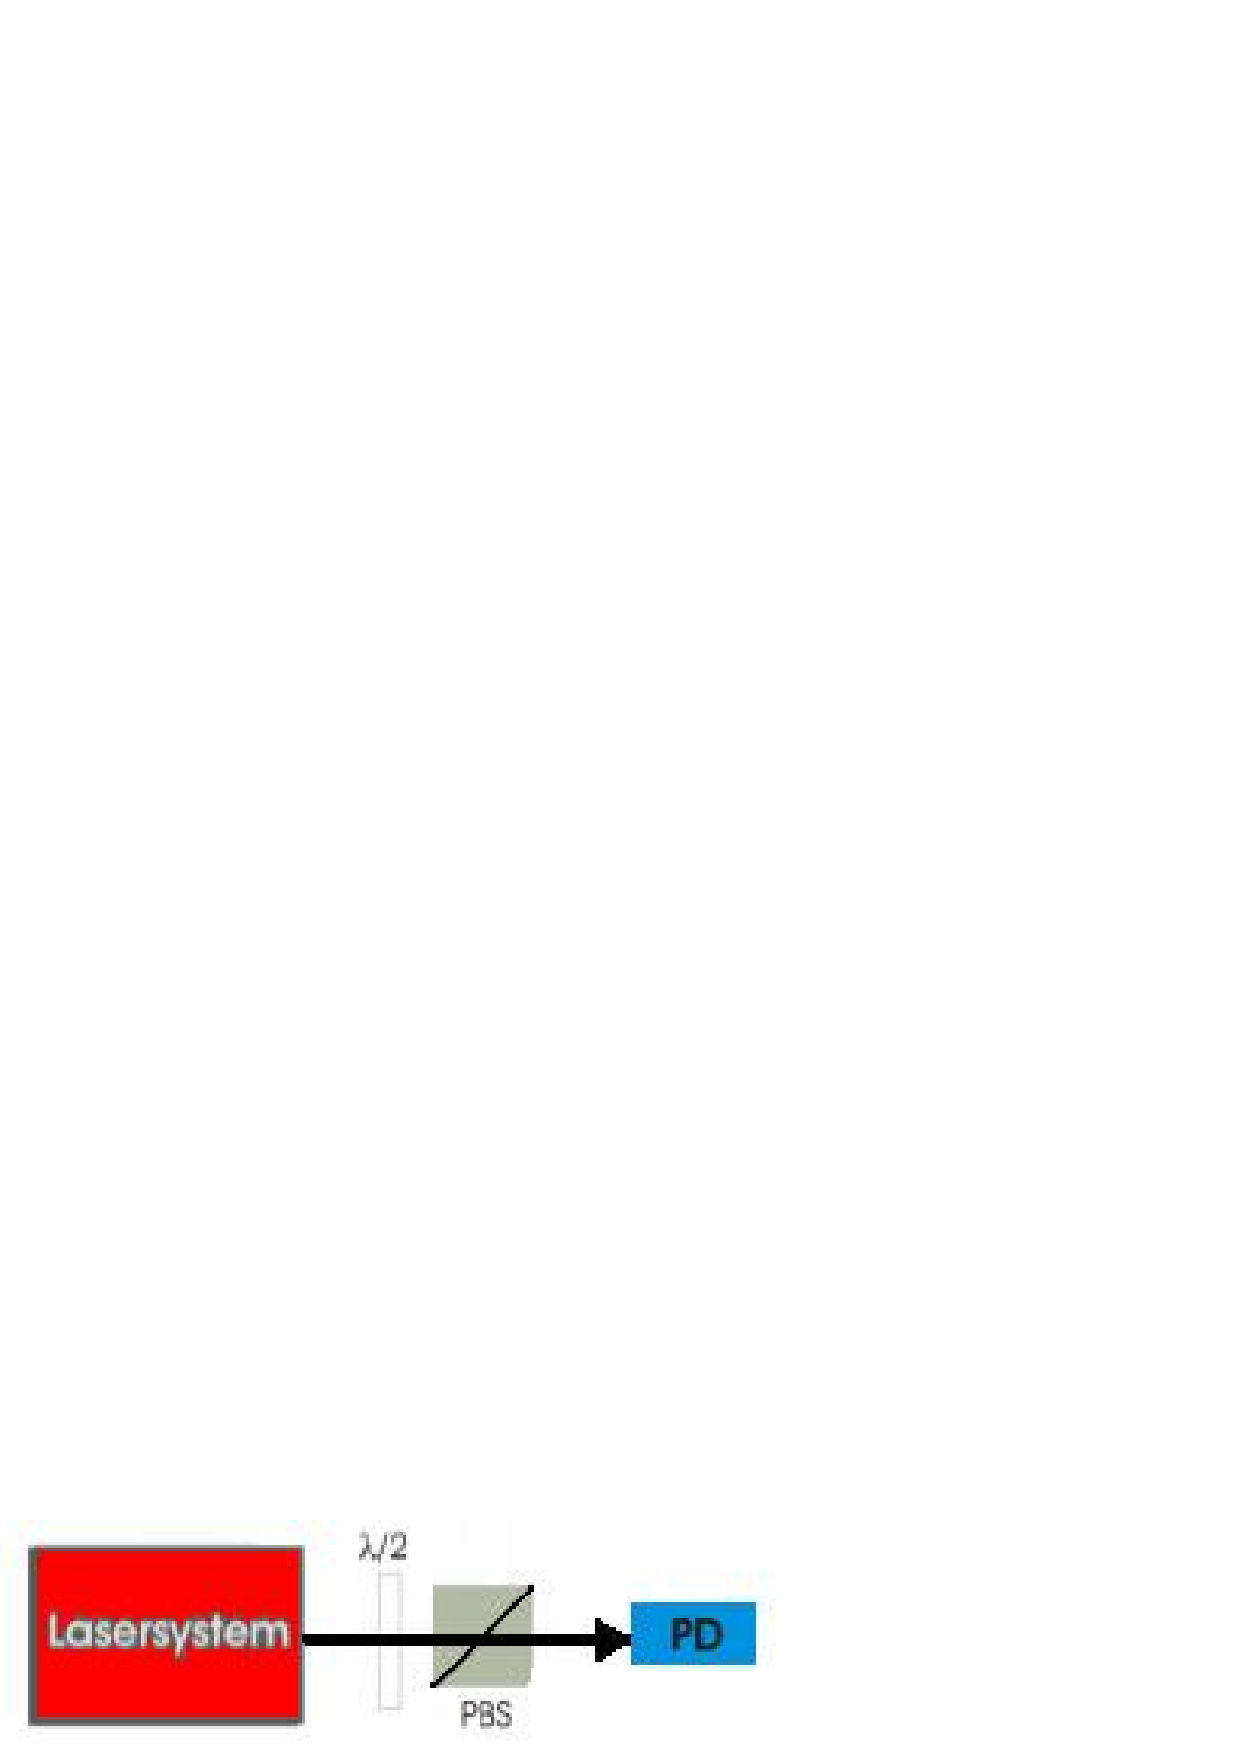
\includegraphics[bb=0 0 379 116]{./pics/eichung_der_photodiode.png}
 % eichung_der_photodiode.png: 505x155 pixel, 96dpi, 13.36x4.10 cm, bb=0 0 379 116
 \caption[Photodiodeneichung]{Versuchsaufbau zur Eichung der Photodiode}
 \label{Photodiodeneichung}
\end{figure}

\subsection{Versuchsdurchführung}


wählen 780.2 nm linie aus
$\alpha=45$\textdegree
$d=0.56 \mu m$
$1800\nicefrac{Linie}{mm}$

\subsection{Auswertung}
\subsection{Ergebnis}


\section{Experiment am Resonator/ Frequenzmodulation}
Für die spätere Spektroskopie sind die Eigenschaften des Resonator entscheident. Deshalb beschäftigen wir uns hier kurz mit ihm. Wir beabsichtigen den freien Spektralbereich, die Länge des Resonator und dessen Finesse zu bestimmen. Haben wir dies geschafft, können wir die Piezo-Frequenz-Charakteristik der Laserdiode aufnehmen, sowie die Frequenzmodulation charakterisieren.

\subsection{Versuchsaufbau}
\begin{figure}
 \centering
 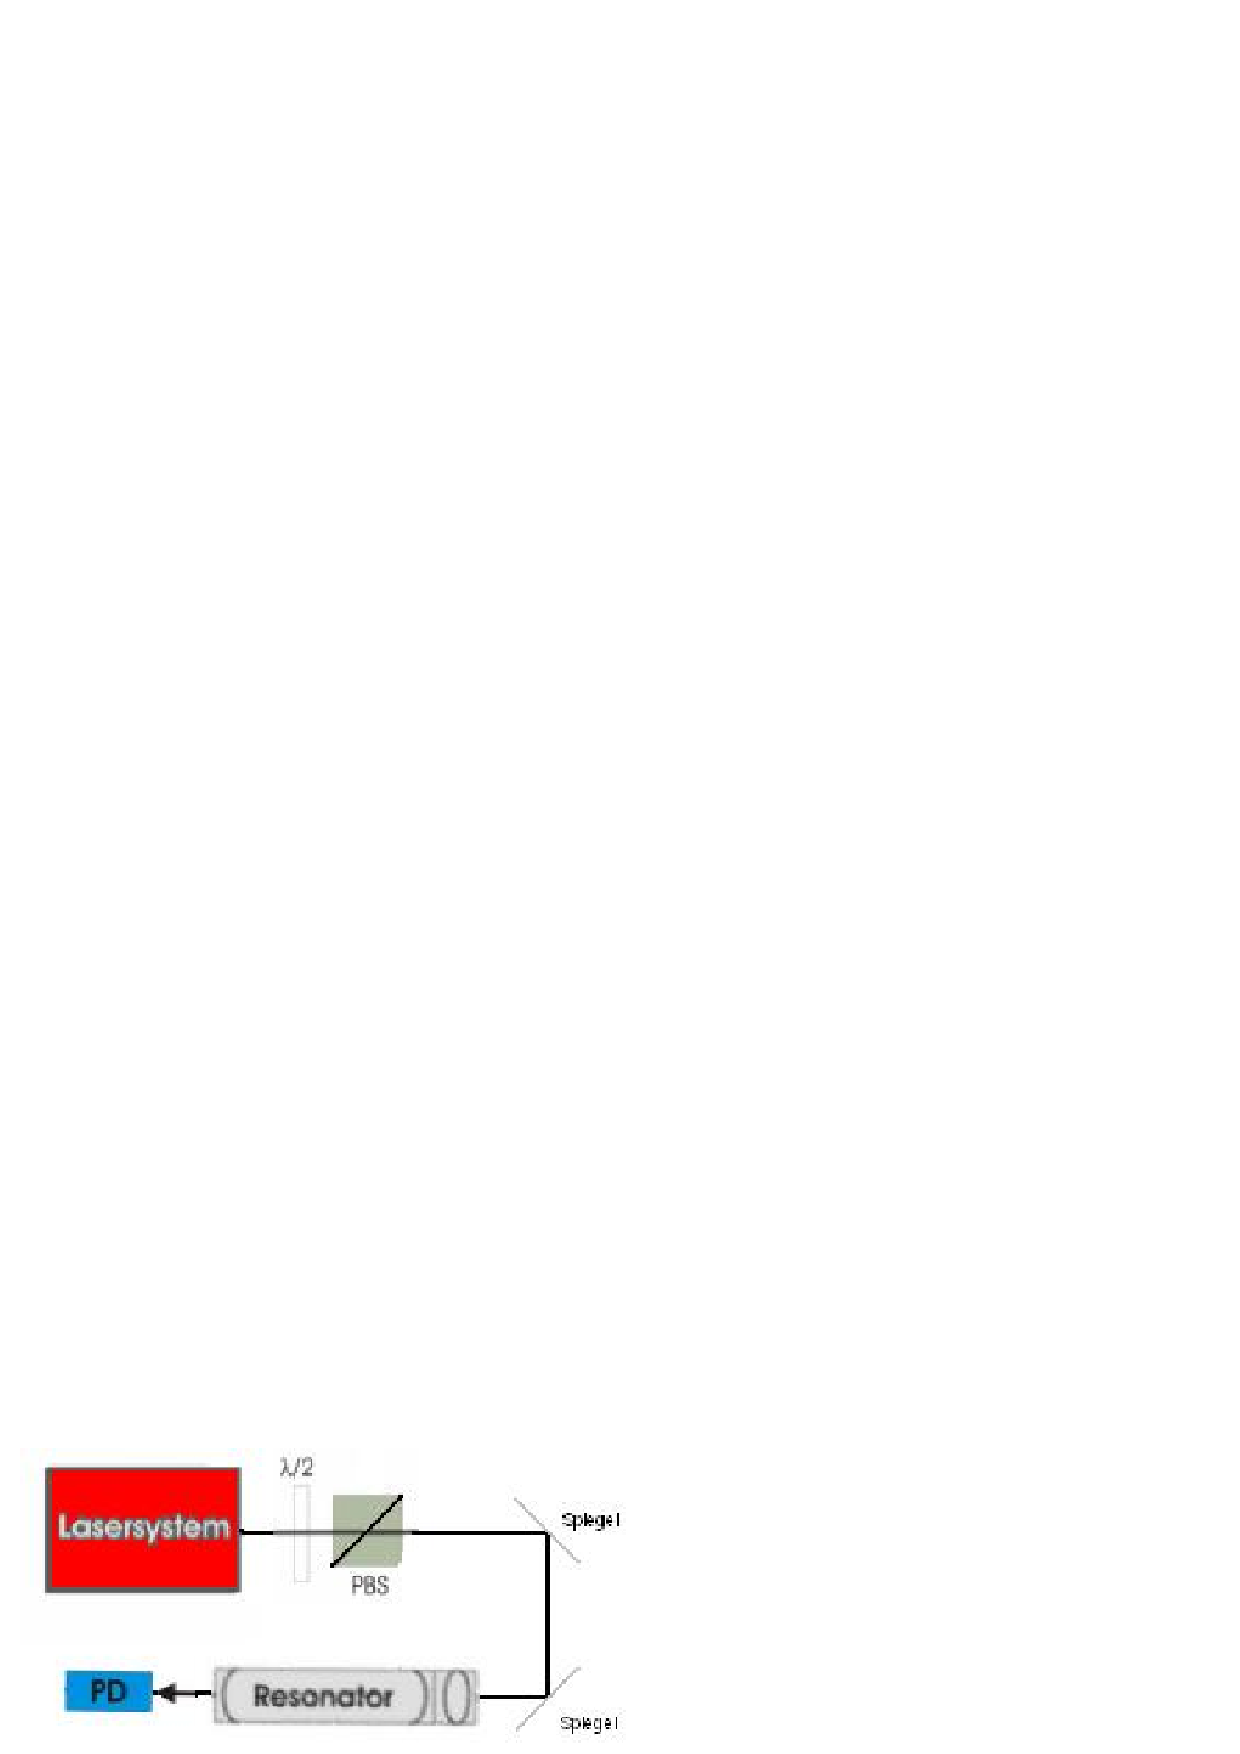
\includegraphics[bb=0 0 313 149]{./pics/experiment_am_resonator.png}
 % experiment_am_resonator.png: 418x199 pixel, 96dpi, 11.06x5.26 cm, bb=0 0 313 149
 \caption{Versuchsaufbau für die Experimente am Resonator}
 \label{Experiment_am_Resonator}
\end{figure}
Der Aufbau findet gemäß Abb \ref{Experiment_am_Resonator} statt.\\
Wir drehen unseren Strahl und filtern ihn danach mit dem PBS um einen linear polarisierten Strahl in die gewünschte Richtung zu erhalten. Die beiden Spiegel benötigen wir um den Strahl in den Resonator einzukoppeln (mehr dazu im \ref{Durchführung_Resonator}).


\subsection{Versuchsdurchführung}
\label{Durchführung_Resonator}
Beamwalk??
\subsection{Auswertung}
\subsection{Ergebnis}


\section{Spektroskopiemethoden}
Jetzt kommen wir zu dem eigentlichen Höhepunkt. Es soll mit drei verschieden Spektroskopiemethoden Aufklärung an einer Rubidiumzelle betrieben werden.
\subsection{Dopplerverbreiterte Laserspektroskopie}
\subsubsection{Prinzip}
Der Hauptstrahl durchläuft die Rb- Zelle und wird dahinter mit einer Photodiode detektiert. Fährt man nun die Frequenz durch, so wird sich bei der Resonazfrequenz der Rb-Atome ein deutlicher Intensitätsverlust am der Photodiode zeigen.\\
Bevor der Strahl allerdings in die Zelle geleitet wird, wird mit einer $\nicefrac{\lambda}{2}$-Plättchen-PBS-Kombination ein schwacher Referenzstrahl abgezweigt. Diesen brauchen wir um den Intesnsitätsverlust auf Grund der Modulation des Laserdiodenstroms $I_{LD}$ ``wegzurechenen''. Hierfür gibt es eine spezielle Mathe- Einheit.\\
Um die Absorptionssignale von der Intensitätsrampe zu trennen, zieht man das Referenzsignal vom Spektroskopiesignal ab. Man normiert quasi das Ausgangssignal auf das Eingangssignal!

\subsubsection{Versuchsaufbau}

\begin{figure}
 \centering
 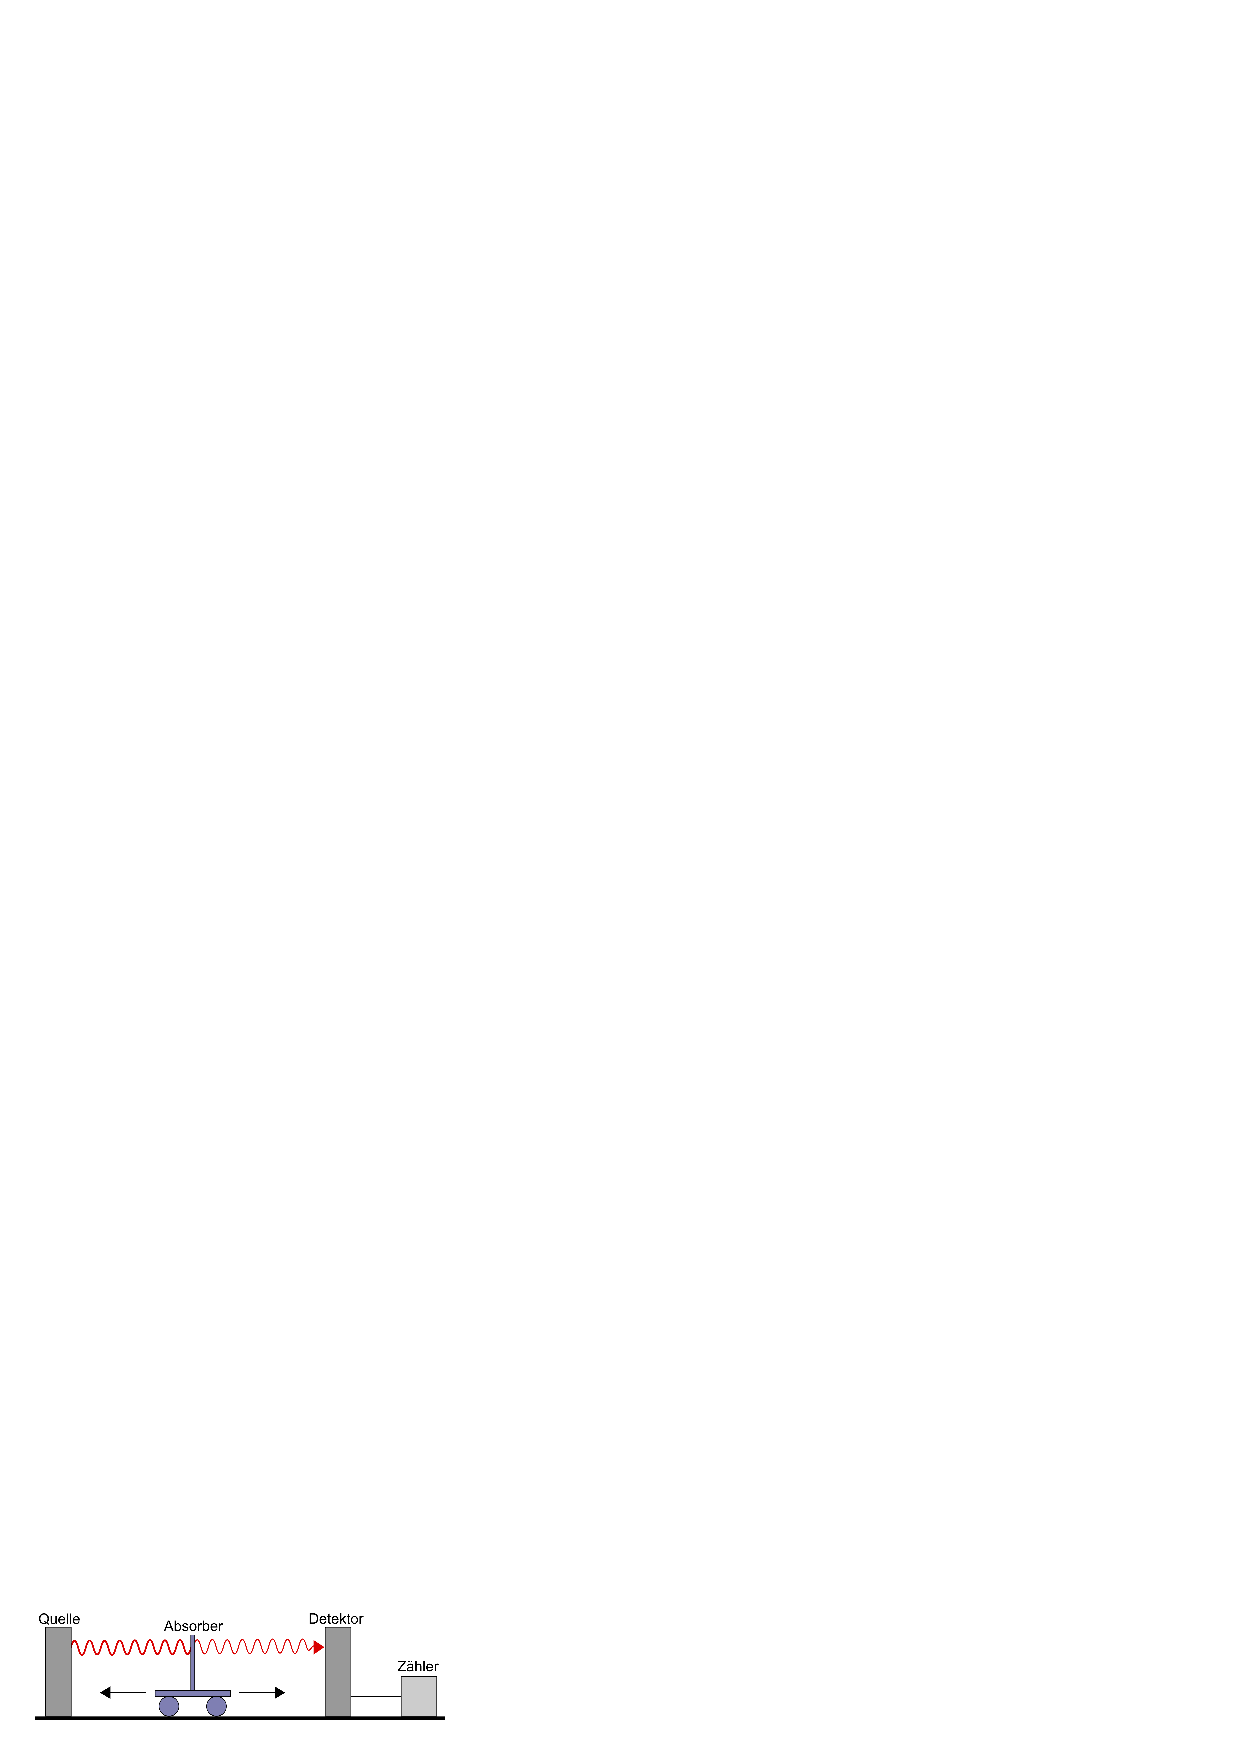
\includegraphics[bb=0 0 321 288]{./pics/aufbau_doppler.png}
 % aufbau_doppler.png: 428x384 pixel, 96dpi, 11.32x10.16 cm, bb=0 0 321 288
 \caption[dopplerverbreiterte Spektroskopie]{Versuchsaufbau für die dopplerverbreiterte Spektroskopie}
 \label{dopplerverbreiterte_Spektroskopie}
\end{figure}


Der Aufbau findes gemäß Abb \ref{dopplerverbreiterte_Spektroskopie} statt. Beim Einsetzen der Zelle in den vorjustierten Laserstrahl ist darauf zu achten, dass der Strahl die Zelle leicht schief durchläuft. Das verhindert unnötige Reflexionen beim Ein- und Austreten.\\
Das Spektroskopiesignal wird auf den ``PD1''- Eingang der Mathe- Einheit gegeben. ``Mon1'' ist ein Monitorausgang, über den man sich das Signal am Oszilloskop ansehen kann. Dieses erscheint invertiert, weil die Schaltung einen invertierenden Verstärker beinhaltet.\\
Das Referenzsignal wird auf den ``PD2''- Eingang gegeben. Über den Monitorausgang ``Mon2'' kann man sich das ebenfalls invertierte Signal ansehen und mit dem zusätzlichen Drehpotentiometer ``Gain'' die Verstärkung einstellen. Um nun die beiden Signale aufeinander abzustimmen, überlagert man die beiden Monitorsignale auf dem Oszilloskop und passt das Referenzsignal über das $nicefrac{\lambda}{2}$-Plättchen vor dem Strahlteiler und über den ``Gain''- Drehpotentiometer an. Das Differenzsignal, das durch eine weitere Invertierung wieder das richtige Vorzeichen hat, kann nun über den Ausgang ``Out'' an das Oszilloskop angeschlossen und nochmal optimiert werden.\\
Das Gerät hat einen weiteren Eingang ``PD3'' mit einem Monitorausgang ``Mon3''. Das Differenzsignal wird durch das an ``PD3'' anliegende Signal geteilt und dann an ``OUT'' ausgegeben. Wenn man diesen ``PD3''- Eingang nicht benutzt, muss der Schalter auf eine über ``Gain'' regelbare Spannungsquelle ``$1-5$ Volt'' umgestellt werden, damit das angeschlossene Signal nicht durch Null geteilt wird. Mit dem Drehpotentiometer ``Offset'' kann das Endsignal vertikal verschoben werden, indem man ihm eine zusätzliche Spannung von $0\cdots10V$ aufaddiert.

\begin{figure}
 \centering
 \includegraphics[bb=0 0 319 208]{./pics/Mathe.png}
 % Mathe.png: 426x278 pixel, 96dpi, 11.27x7.35 cm, bb=0 0 319 208
 \caption{Mathe- Einheit}
\end{figure}
\begin{figure}
 \centering
 \includegraphics[bb=0 0 387 212]{./pics/Schaltplan_mathe.png}
 % Schaltplan_mathe.png: 646x353 pixel, 96dpi, 17.09x9.34 cm, bb=0 0 484 265
 \caption{Schaltplan der Mathe- Einheit}
\end{figure}

\subsubsection{Versuchsdurchführung}
feed forward, fingerkamerad,...
\subsubsection{Auswertung}
\subsubsection{Ergebnis}

\subsection{Dopplerfreie Spektroskopie}
Die Linienbreite der atomaren Resonanzlinien wird bei Zimmertemperatur durch den Doppler- Effekt dominiert. Man würde gerne Atome mit der Geschwindigkeit $v=0$ spektroskopieren. Das ist mit der Technik der \textbf{Sättigungsspektroskopie} auch möglich. Dadurch können wir die Hyperfeinstruktur messen. Der Trick hierbei ist, einen Sättigungsstrahl und einen entgegenlaufenden Abfragestrahl zu verwenden.\begin{figure}
 \centering
 \includegraphics[bb=0 0 439 96]{./pics/abfragestrahl.png}
 % abfragestrahl.png: 585x128 pixel, 96dpi, 15.48x3.39 cm, bb=0 0 439 96
 \caption{Sättigungs- und Abfragestrahl}
\end{figure}

\subsubsection{Prinzip}
Betrachten wir der Einfachheit halber erst einmal ein Zwei- Niveau- System mit einem Grundzustand $\ket{G}$ und einem angeregten Zustand $\ket{A}$.\\
Die Atome in der Gaszelle unterliegen der Maxwellschen Geschwindigkeitsverteilung. Uns interessiert nur die Geschwindigkeit in Richtung des Laserstrahles, die eine Gaußkurve darstellt. Strahlt man dmit Laserlicht in die Zelle, dessen Frequnz $\omega_L$ etwas kleiner ist als die atomare Resonanzfrequenz $\omega_0$, so wird dieser Strahl nur von den Atomen asorbiert, die ihm mit der richtigen Geschwindigkeit $-v_x$ entgegenfliegen. Es gilt: $\omega_L=\omega_0-kv_x$.\\
Ein zurücklaufender (gespiegelter) Strahl wird von den Atomen dieser Geschwindigkeitsklasse nicht beeinflusst, sondern von den Atomen der Geschwindigkeitsklasse $+v_x$ absorbiert. Strahlt man jedoch in der Resonanzfrequenz $\omega_0$ in die Rb-Zelle ein, so werden die Atome mit Geschwindigkeitskomponente $v_x=0$ angeregt. Der reflektierte Abfragestrahl durchläuft das Medium dann mit geringerer Absorption.\\
\begin{figure}
 \centering
 \includegraphics[bb=0 0 295 153]{./pics/lambdip.png}
 % lambdip.png: 393x204 pixel, 96dpi, 10.40x5.40 cm, bb=0 0 295 153
 \caption{Absorptionslinie mit Lambdip}
\end{figure}
Man bekommt somit schmale dopplerfreie Resonanzlinien im dopplerverbreiterten Untergrund. Diese tragen den Namen \textbf{Lambdips}. Leider ist das nicht das Ende vom Lied, denn wir haben schließlich kein reines Zwei- Niveau- System vorliegen. Nehmen wir an, dass wir 2 Übergänge vom Grundzustand $\ket{G}$ in die Anregungszustände $\ket{A_1}$ und $\ket{A_2}$, deren Frequenzabstand $\omega_2-\omega_1$ kleiner als die Dopplerbreite ist, vorliegen haben.\\
Dann treten neben den Lambdips zusätzliche Resonanzen auf, sogenannte \textbf{Crossover-Resonanzen}. Betrachten wir die Frequenz $\omega=\frac{\omega_2+\omega_1}{2}$, bei der der Sättigungsstrahl Atome mit einer Geschwindigkeitskomponente $-v_x$ auf das untere Niveau anregen kann und der Abfragestrahl dieselben Atome (die in seinem System die Geschwindigkeit $+v_x$ haben) auf das obere Niveau anregen kann. Es gilt dann:
\begin{equation}
 \omega_1-kv_x=\omega_2+kv_x\;\;\;\;\Longrightarrow\;\;\;\;\; kv_x=\frac{\omega_2-\omega_1}{2}
\end{equation}
Der Sättigungsstrahl erzeugt eine Abnahme der Besetzungsdichte im gemeinsamen unteren Niveau. Dadurch wird das Medium für den Abfragestrahl transparent. Das zu erwartende Sättigungsspektrum ist an Hand eines einfachen Beispiels in Abb. \ref{saettigungsspektrum} skizziert.
\begin{figure}
 \centering
 \includegraphics[bb=0 0 313 284]{./pics/crossover.png}
 % crossover.png: 418x379 pixel, 96dpi, 11.06x10.03 cm, bb=0 0 313 284
 \caption[Crossoverresonanz]{Entstehung der Lambdips und Crossover- Resonanzen für einen Grundzustand un zwei angeregt Zustände $\ket{A_1}$ und $\ket{A_2}$. Die ruhenden Atome sehen die Resonanzfrequenz und es kommt zu Lambdips. Die Geschwindigkeitsklasse des Abfragestrahls für den Übergang $\ket{G}\rightarrow\ket{A_1}$ wechselwirkt mit derjenigen des Sättigungsstrahls für den Übergang $\ket{G}\rightarrow\ket{A_2}$, wodurch es zu Crossover- Resonanzen kommt}
\end{figure}



\subsubsection{Versuchsaufbau}
\begin{figure}
 \centering
 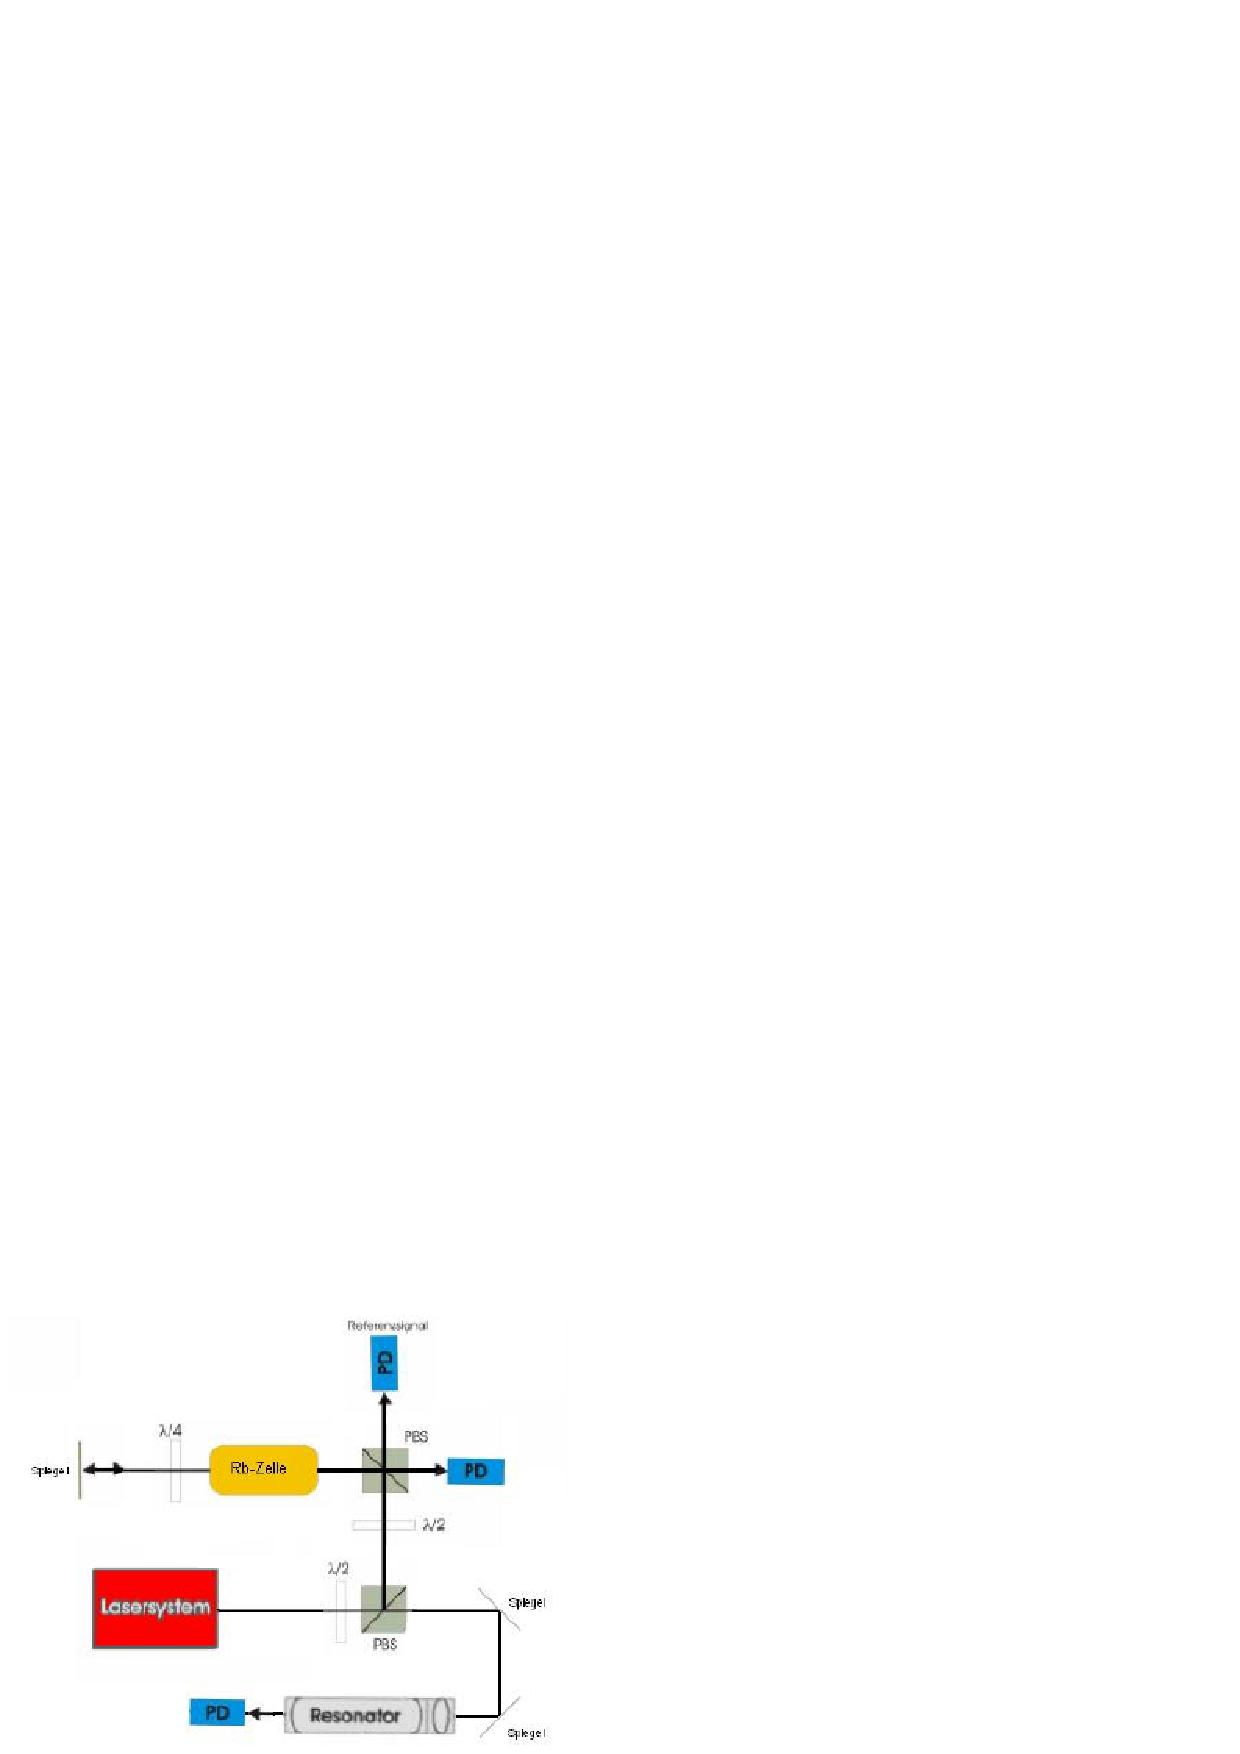
\includegraphics[bb=0 0 281 211]{./pics/aufbau_dopplerfrei.png}
 % aufbau_dopplerfrei.png: 375x281 pixel, 96dpi, 9.92x7.43 cm, bb=0 0 281 211
 \caption[Dopperfreie Spektroskopie]{Versuchsaufbau für die dopplerfreie Spektroskopie}
 \label{aufbau_dopplerfrei}
\end{figure}
Der Versuchsaufbau ist ähnlich der dopplerverbreiterten Spektroskopie. Es wird lediglich die Photodiode hinter der Rb- Zelle mit einen Spiegel vertauscht und die Photodiode gegenüber angebracht (siehe Abb. \ref{aufbau_dopplerfrei}).

\subsubsection{Versuchsdurchführung}
\subsubsection{Auswertung}
\subsubsection{Ergebnis}


\subsection{FM-Spektroskopie}
Bei sehr kleinen Absorptionen ist die Methode der Absorptionsmessung, nicht genau genug. Daher sind verschiedene Verfahren entwickelt worden, die oft eine Steigerung der Nachweisempfindlichkeit um viele Größenordnungen erlauben. Im folgenden soll eine davon, nämlich die FM-Spektroskopie vorgestellt werden.\\
Mit ihr ist es möglich die Ableitung der Resonazlinien, die beim Peak einen Nulldurchgang haben, sichbar zu machen und damit die Empfindlichkeit zu steigen.
\subsubsection{Prinzip}
Der Laserfrequenz wird eine Hochfrequnz aufmoduliert. Das gemessene Signal wird mit dem Signal des VCOs, dem eine zusätzliche Phasenverschiebung addiert wird, gemischt und durch einen Tiefpass geleitet, der die hochfrequenten Terme herausfiltert.

\subsubsection{PrinzipII}
Moduliert man die Laserfrequenz $\omega_0$ mit einer Hochfrequenz $\omega_M$, so ergibt sich für das vom Laser emitierte Lichtfeld (siehe \ref{theorie_fm}):

\subsubsection{Versuchsaufbau}
\subsubsection{Versuchsdurchführung}
\subsubsection{Auswertung}
\subsubsection{Ergebnis}


\section{Messung der Polarisation von Licht}

\section{Magneto- optische Effekte}


$\bra{hallo}
\ket{servus}$




%*****************************************************************

%*****************************************************************
\clearpage
\appendix
\section{Fragen zur Vorbereitung}
\subsection{Das Lasersystem}
\begin{itemize}
 \item Was ist ein Modensprung?
\end{itemize}
Von einem Modensprung spricht man, wenn sich die Anzahl der Knoten der stehenden Welle in Resonator ändert.
\begin{itemize}
 \item Was versteht man unter einem Piezo?
\end{itemize}
Ein Piezo ist ein elektrisches Bauteil, welches seine Abmessung beim anlegen einer Spannung verändert. Diese Abhängigkeit ist sehr empfindlich und eignet sich deshalb hervorragend um kleine Verschiebungen zu realisieren.

\begin{itemize}
\item Wie funktioniert ein PID- Regler?
\end{itemize}
Der PID- Regler benutzt 3 unahängige Parameter: den Proportionalwert,den Integral- und den Ableitungswert. Der Proportionalwert bestimmt die Reaktion auf die aktuelle Abweichung, der Integralwert bestimmt die Antwort auf die Summe aller bisherigen Fehler und der Ableitungswert schließlich wird der Änderungsrate des Fehlers von ``Ist''- Wert gerecht.\\
Das gewichtete Mittel dieser 3 wird verwendet, um den Prozess mittels einer Steuerung auf dem ``Soll''- Wert zu halten.
\begin{itemize}
\item Warum benutzt man ein Prismenpaar?
\end{itemize}
Um das ellipsenförmige Strahlprofil der Laserdiode symmetrisch zu machen.

\subsection{Der Resonator}
\begin{itemize}
\item Wieso braucht man zwei Spiegel, um in den Resonator einzukoppeln?
\end{itemize}
Um den Laser mit der Methode des \textbf{Beamwalks} justieren zu können.
\begin{itemize}
\item Warum sollte bei einem Resonator die Finesse möglichst groß sein?
\end{itemize}
Um eine möglichst große Auflösung zu erhalten.
\begin{itemize}
\item Warum werden die Scans mit einem Dreieck- und nicht mit einem sinusförmigen Signal durchgeführt?
\end{itemize}
Weil die Abhängigkeit auch linear ist?

\begin{itemize}
\item Welche Scan- Möglichkeiten gibt es, um die Cavity- Peaks zu sehen?
\end{itemize}
\subsection{Eigenschaften von Rubidium}
\begin{itemize}
\item Welche Auswirkungen hat die Existenz der beiden Isotope auf das Absorptionsspektrum?
\end{itemize}
Es wird verschmiert.

\begin{itemize}
\item Warum ist der optische Übergang von 
$5^2P_{\nicefrac{3}{2}}\longrightarrow5^2P_{\nicefrac{1}{2}}$
nicht erlaubt?
\end{itemize}
Bei diesem Übergang ist der Drehimpuls erhalten!!! Falls ein optischer Übergang statt finden soll, muss das wegfliegende Photon aber ebenfalls Drehimpuls mit sich tragen, da es sich um ein Spin $1$ Teilchen handelt. Die Auswahlregel eines optische Überganges ($\Delta l=\pm1$) ist verletzt.

\subsection{Linienverbreiterungen und Absorptionsquerschnitt}
\begin{itemize}
\item Welche Arten von Linienbreiten gibt es bei optischen Übergängen zwischen Energieniveaus? Welche dominiert bei Rubidium- Dampf bei Zimmertemperatur?
\end{itemize}
Natürliche Linienbreite, Doppler- Verbreiterung, Stoßverbreiterung, Sättigungsverbreiterung, Flugzeitlinienbreite.\\
Beim Rubidum- Dampf dominiert die Doppler- Verbreiterung.
\begin{itemize}
\item Leite die Halbwertsbreite der dopplerberbreiterten Linien aus der Maxwell- Boltzmann- Verteilung ab!
\end{itemize}
Die Maxwell-Bolzmann- Verteilung ist gegeben durch:
\begin{equation}
 n_i(v_z)dv_z=\frac{N_i}{v_w\cdot \sqrt{\pi}} e^{-(\nicefrac{v_z}{v_w})^2}dv_z
\end{equation}
wobei $v_w=\sqrt{\nicefrac{2k_bT}{m}}$ und $N_i=\int_{-\infty}^{+\infty}n_i(v_z)dv_z$ sind.\\
Wir verwenden jetzt die Beziehung (\ref{doppler_beziehung}) und ersetzten
\begin{equation}
 v_z=c(\frac{\omega}{\omega_0}-1)\;\;\;\;\;\text{und}\;\;\;\;\;dv_z=(\nicefrac{c}{\omega_0})d\omega
\end{equation}
\begin{equation}
 \Longrightarrow n_i(\omega)d\omega=\frac{c\cdot N_i}{\omega_0\cdot v_w\cdot \sqrt{\pi}} e^{-[\nicefrac{c(\omega-\omega_0)}{(\omega_0\cdot v_w)}]^2}
\end{equation}
Die Halbwertsbreite ist die Stelle für die gilt:
\begin{equation}
 P(\omega_1)=P(\omega_2)=\frac{1}{2}P(\omega_0)
\end{equation}
Noch die Definition von $v_w$ einsetzen und es folgt sofort Gleichung (\ref{Doppler})
\begin{equation*}
 \Delta \omega_{Doppler}=\left(\nicefrac{\omega_0}{c}\right)\sqrt{\nicefrac{8k_B T\cdot \ln(2)}{m}}
\end{equation*}

\begin{itemize}
\item Welche Dopplerbreite erwartet man für eine Linie bei Zimmertemperatur ($\lambda=780.2nm$, mittlere Atommasse: $m(Rb)=85.4678u$)?
\end{itemize}
Das elementare Zahlen einsetzten für auf einen Wert in Einheiten der Kreisfrequenz von $3.24 GHz$.
\begin{itemize}
\item Berechne die Teilchendichte $n$ in der Rb- Zelle!
\end{itemize}
\begin{equation}
 n=\frac{N}{V}
pV=nRT V noch nicht bekannt messen!!!
\end{equation}

\begin{itemize}
\item Wie groß ist der Absorptionsquerschnitt für Rubidium nach der Näherungsformel?
\end{itemize}

\begin{itemize}
\item Welcher Teil der Intensität wird also absorbiert?
\end{itemize}

\subsection{FM- Spektroskopie}
\begin{itemize}
\item Man ändert die Phase $\phi$ um $180$\textdegree. Wie ändert sich dabei das Signal $U_{End}$?
\end{itemize}

\begin{itemize}
\item Welche Zeitverzögerung (in $ns$) entspricht bei einer Modulationsfrequenz von $\omega_M=50 MHz$ bzw. $\omega_M=100 MHz$ einer Änderung der Phase von $90$\textdegree bzw. $180$\textdegree?
\end{itemize}

\subsection{Jones- Vektoren}
\begin{itemize}
\item Wie sehen Jones- Vektoren für horizontales und vertikales lineares Licht aus?
\end{itemize}
\begin{equation}
 \text{Lineare Polarisation in $x$-Richtung: }
\left(\begin{array}{c}
       1\\
0
      \end{array}
\right)
\end{equation}

\begin{equation}
 \text{Lineare Polarisation in $y$-Richtung: }
\left(\begin{array}{c}
       0\\
1
      \end{array}
\right)
\end{equation}


\begin{itemize}
\item Wie sehen Jones- Vektoren für lineares Licht unter einem Winkel $\gamma$ aus?
\end{itemize}
\begin{equation}
 \text{Lineare Polarisation in $x$-Richtung: }
\left(\begin{array}{c}
       \cos(\gamma)\\
      \sin(\gamma)
      \end{array}
\right)
\end{equation}


\begin{itemize}
\item Wie sehen Jones- Vektoren für zirkulares Licht aus?
\end{itemize}
\begin{equation}
 \text{Rechtszirkulares Licht: }\sigma^+=\frac{1}{\sqrt{2}}
\left(\begin{array}{c}
       1\\
i
      \end{array}
\right)
\end{equation}
\begin{equation}
 \text{Linkszirkulares Licht: }\sigma^-=\frac{1}{\sqrt{2}}
\left(\begin{array}{c}
       1\\
i
      \end{array}
\right)
\end{equation}
\begin{itemize}
\item Welche anderen Phasenunterschiede ausser $\nicefrac{\pi}{2}$ führen zu zirkularem Licht?
\end{itemize}
Sowohl die positiven ganzzahlingen Vielfachen von $\nicefrac{\pi}{2}$ als auch die Negativen.
\begin{itemize}
\item Mit welchen 3 Größen kann man den Polarisationszustand eindeutig bestimmen? Welche Form hat dieser im allgemeinen?
\end{itemize}
Wir benötigen einen Vektor auf den komplezen Einheitskreis (2 Größen) und eine beliebiege komplexe Phase. Im allgemeinen ist diese Phase sicher nicht $0$ und auch kein ganzzahliges Vielfaches von $\nicefrac{\pi}{2}$. Deshalb ist das Licht unpolarisiert.
\subsection{Jones- Matrizen}
\begin{itemize}
\item Überlegen sie sich dies und verfizieren sie dabei
\end{itemize}
$$ \bf{T}_{\frac{\lambda}{2}}(\alpha) = \left( \begin{array}{cc}
\cos (2\alpha)&\sin (2\alpha) \\
\sin (2\alpha)&-\cos (2\alpha)
\end{array} \right) $$
\begin{itemize}
\item Wie transformiert sich lineares Licht unter einem Winkel $\gamma$ zur $x$-Achse durch ein solches $\frac{\lambda}{2}$- Plättchen?
\end{itemize}
\begin{itemize}
\item Wie sieht die Jones- Matrix für ein $\frac{\lambda}{4}$- Plättchen unter einem Winkel von $0$\textdegree aus? Überlegen Sie sich dies analog zu 3.8.
\end{itemize}
\begin{itemize}
\item Verifizieren Sie, dass ein $\frac{\lambda}{4}$-Plättchen unter einem Winkel von $\alpha$ durch folgende Matrix beschrieben wird:
\end{itemize}
$$\bf{T}_\frac{\lambda}{4}(\alpha)=\frac{1}{\sqrt{2}}
\left(
\begin{array}{cc}
 1-i\cos(2\alpha)&-i\sin(2\alpha)\\
-i\sin(2\alpha)&1+i\cos(2\alpha)
\end{array}
\right)
$$

\begin{itemize}
\item Wie lauten die Basisvektoren für horizontales und vertikales lineares Licht und wie transformieren sie sich durch ein $\frac{\lambda}{4}$- Plättchen unter $45$\textdegree?
\end{itemize}


\clearpage
\section{Optische Elemente}
\subsection{PBS}
\label{pbs}

spielen

\begin{pgfpicture}{0cm}{0cm}{5cm}{2cm}
  %\pgfputat{\pgfxy(1,1)}{\pgfbox[center,center]{Hi}}
  % pgfputat places something at a certain position
  % pgfbox shows the text ‘hi!’. The horizontal alignment
  % is centered (other options: left, right). The vertical
  % alignment is also centered (other options: top, bottom,
  % base).
  %\pgfcircle[stroke]{\pgfxy(1,1)}{0.5cm}
  
  % In the following, all lines will end with an arrow that looks like
  % the arrow of TeX’s \to command
  %\pgfputat{\pgfxy(3,1)}
    \begin{pgfrotateby}{\pgfdegree{90}}
      % You can rotate things like this
      \pgfbox[center,center]{$\int_0^\infty xdx$}
    \end{pgfrotateby}
  %\pgfcircle[stroke]{\pgfxy(4,1)}{1cm}
  \pgfnodecircle{Node1}[stroke]{\pgfxy(1,0.5)}{0.25cm}
\pgfnodecircle{Node2}[stroke]
  {\pgfrelative{\pgfxy(1,0)}{\pgfnodecenter{Node1}}}{0.25cm}
\pgfnodecircle{Node3}[stroke]
  {\pgfrelative{\pgfxy(1,0)}{\pgfnodecenter{Node2}}}{0.25cm}
\pgfnodecircle{Node4}[stroke]
  {\pgfrelative{\pgfxy(1,0)}{\pgfnodecenter{Node3}}}{0.25cm}

\end{pgfpicture}


\listoffigures

%*****************************************************************
\nocite{anl}




\end{document}
